\documentclass[aspectratio=169]{beamer}

\usepackage{amsmath,amssymb}
\usepackage{booktabs}
\usepackage{tabularx}
\usepackage{colortbl}
\usepackage{tikz}
\usetikzlibrary{arrows.meta,backgrounds,calc,positioning,shapes.multipart,fit}
\usepackage[main=english]{babel}
\usepackage{ragged2e}

\definecolor{fortranPurple}{HTML}{503874}  % poster deep purple
\definecolor{fortranPurpleMid}{HTML}{7E5AA6}
\usetheme[
  accent=fortranPurple,
  progressbar=foot,
  sectionpage=progressbar,
  subsectionpage=progressbar,
  numbering=fraction,
  numberrail=section,
  block=fill,
  notes=hide,
  toc=aftertitle,
  closing=contact
]{cookie}

% \yes/\prt/\nope and cDone/cWip/cTodo are defined by compiler_table.tex

% complexity badge helper
\newcommand{\cplx}[1]{{\footnotesize\color{cookieMuted}#1}}

% Widen the footer author box so the three institutions fit (default is .18\paperwidth)
\makeatletter
\setbeamertemplate{footline}{%
  \leavevmode\vbox{%
    \ifdefstring{\cookie@progressbar}{foot}{\hbox{\cookie@progressrule{\paperwidth}}}{}%
    \hbox{%
      \begin{beamercolorbox}[wd=.36\paperwidth,ht=2.7ex,dp=1.15ex,leftskip=.02\paperwidth]{footline}%
        \usebeamerfont{footline}\insertshortauthor
      \end{beamercolorbox}%
      \begin{beamercolorbox}[wd=.46\paperwidth,ht=2.7ex,dp=1.15ex,leftskip=.012\paperwidth,rightskip=.012\paperwidth]{footline}%
        \usebeamerfont{footline}\insertshorttitle%
        \ifx\insertsectionhead\@empty\else\hfill\cookie@footersection{\insertsectionhead}\fi%
      \end{beamercolorbox}%
      \begin{beamercolorbox}[wd=.18\paperwidth,ht=2.7ex,dp=1.15ex,leftskip=.027\paperwidth,rightskip=.014\paperwidth plus 1fil]{footline right}%
        \usebeamerfont{footline number}\strut\cookie@insertnumber
      \end{beamercolorbox}%
    }%
  }%
}
% 7 sections overflow the single-column agenda: split into two columns above 6
\expandafter\patchcmd\csname\string\cookie@agendarendertoc\endcsname{>8}{>6}{}{\PackageWarning{deck}{agenda patch failed}}
\makeatother

\usepackage[utf8]{inputenc}
\usepackage{pgfplots}
\pgfplotsset{compat=1.18}
\usepackage{braket}
\usepackage{siunitx}
\usepackage[version=4]{mhchem}
\usetikzlibrary{decorations.pathreplacing,patterns,shapes.geometric,3d}

% dashed placeholder for photos Jorge should drop in
\newcommand{\figph}[3][]{%  [opts] {width}{description}
  \begin{tikzpicture}
    \node[draw=cookieMuted,dashed,line width=.8pt,minimum width=#2,minimum height=#2*0.55,
          text width=#2-1em,align=center,font=\scriptsize\color{cookieMuted},#1]{[FOTO] #3};
  \end{tikzpicture}}
\newcommand{\src}[1]{{\tiny\color{cookieMuted}#1}}
\newcommand{\Eh}{E_\mathrm{h}}
\newcommand{\vr}{\mathbf{r}}
\newcommand{\vR}{\mathbf{R}}

\title[Química computacional]{Química computacional}
\subtitle{Una amalgama de física, matemáticas, química y computación}
\author[Jorge L. Gálvez Vallejo]{Jorge Luis Gálvez Vallejo}
\cookieemail{jorge.galvezvallejo@anu.edu.au}
\institute{NCI \textperiodcentered\ ANU}
\cookieuni{Australian National University}
\cookielocation{Canberra, Australia}
\date{\today}
\cookietagline{Instituto Tecnológico de Ciudad Madero}

\titlegraphic{%
  \begin{tcolorbox}[enhanced,colback=white,colframe=white,boxrule=0pt,
      arc=5pt,width=3.1cm,left=7pt,right=7pt,top=8pt,bottom=8pt,
      halign=center,valign=center,nobeforeafter,box align=center]
    
\includegraphics[height=1.05cm]{assets/nci.png}
  \end{tcolorbox}%
}
\cookieclosingtitle{¡Gracias!}
\cookieclosingtext{Explorando para qué sirve la química computacional, con énfasis cuántico y molecular.}
\cookieclosingqr{https://github.com/JorgeG94}
\cookieclosingqrlabel{github.com/JorgeG94}

\begin{document}

\maketitle

% =====================================================================
\section{¿Qué es la química?}

\begin{frame}{Química}{Estudio de la materia y de su cambio}
  \begin{columns}[T,onlytextwidth]
    \column{.5\textwidth}
      \begin{itemize}\setlength\itemsep{6pt}
        \item \textbf{Primaria:} ``las cosas que se mezclan y huelen feo''
        \item \textbf{Secundaria:} ``la tabla periódica y a balancear ecuaciones''
        \item \textbf{Universidad:} ``\textbf{materia} y sus \textbf{transformaciones}'' \cplx{(y mucho dolor)}
      \end{itemize}
    \column{.46\textwidth}
      \begin{block}{La definición que sí usamos}
        Qué \textbf{es} la materia, cómo se \textbf{enlaza} y cómo \textbf{cambia}.
      \end{block}
      \cplx{Los tres niveles son verdad; solo cambia la resolución.}
  \end{columns}
\end{frame}

\begin{frame}{De átomos a moléculas a propiedades}
  \centering
  \begin{tikzpicture}[x=1cm,y=1cm,
      box/.style={draw=cookieAccent,rounded corners=3pt,thick,minimum width=3.4cm,minimum height=1.5cm,align=center,fill=cookieAccent!8},
      arr/.style={-{Stealth},very thick,cookieAccent}]
    \node[box] (a) at (0,0) {\textbf{Átomos}\\[-1pt]{\scriptsize núcleo + electrones}};
    \node[box] (m) at (4.6,0) {\textbf{Moléculas}\\[-1pt]{\scriptsize enlaces: covalente, iónico\ldots}};
    \node[box] (g) at (9.2,0) {\textbf{Materia}\\[-1pt]{\scriptsize agregados macroscópicos}};
    \draw[arr] (a)--(m); \draw[arr] (m)--(g);
    \node[font=\scriptsize\color{cookieMuted}] at (2.3,-1.0) {enlazan};
    \node[font=\scriptsize\color{cookieMuted}] at (6.9,-1.0) {se agregan};
    \node[draw=cookieMuted,dashed,rounded corners=3pt,text width=3.4cm,align=center,font=\small] at (9.2,-2.6)
      {dureza \quad pH\\ fragilidad \quad color\\ conductividad\ldots};
    \draw[-{Stealth},cookieMuted] (g)--(9.2,-1.95);
  \end{tikzpicture}\\[1.2em]
  \begin{exampleblock}{Idea central}
    Las propiedades que \textbf{medimos} nacen de cómo se comportan los \textbf{electrones}.
  \end{exampleblock}
\end{frame}

\begin{frame}{Modelos de la química}
  \begin{columns}[T,onlytextwidth]
    \column{.5\textwidth}
      \begin{itemize}\setlength\itemsep{6pt}
        \item El entendimiento \textbf{moderno} de la química es relativamente \textbf{nuevo}.
        \item Nace con la era de la \textbf{mecánica cuántica} \cplx{(años 1920)}.
        \item Modelos \textbf{pre-cuánticos}:
          \begin{itemize}
            \item \textbf{Lewis} --- puntos y pares de electrones
            \item \textbf{Bohr} --- órbitas con energía fija
          \end{itemize}
      \end{itemize}
    \column{.46\textwidth}
      \centering
      \begin{tikzpicture}[scale=.95]
        \draw[cookieMuted] (0,0) circle (.55);
        \draw[cookieMuted] (0,0) circle (1.05);
        \draw[cookieMuted] (0,0) circle (1.6);
        \fill[cookieAccent] (0,0) circle (.12);
        \fill[cookieAccent!70] (.55,0) circle (.07);
        \fill[cookieAccent!70] (-.74,.74) circle (.07);
        \fill[cookieAccent!70] (1.13,-1.13) circle (.07);
        \draw[-{Stealth},cookieAccent,thick] (1.13,-1.13)--(.74,-.74) node[midway,right,font=\tiny]{$h\nu$};
        \node[font=\tiny\color{cookieMuted}] at (0,-1.95) {Modelo de Bohr (esquema)};
      \end{tikzpicture}\\[.3em]
      \cplx{Explica el hidrógeno; se rompe con el helio.}
  \end{columns}
\end{frame}

\begin{frame}{Modelo clásico y su ruptura}{La catástrofe ultravioleta}
  \begin{columns}[T,onlytextwidth]
    \column{.5\textwidth}
      \begin{itemize}\setlength\itemsep{4pt}
        \item \textbf{Mecánica estadística} y \textbf{termodinámica estadística}.
        \item Radiación de \textbf{cuerpo negro}: la teoría clásica predice energía \textbf{infinita}.
        \item Planck (1900): la energía viene en \textbf{cuantos}.
      \end{itemize}
      \[ E = h\nu \]
      \[ u(\nu,T)=\frac{8\pi h\nu^{3}}{c^{3}}\,\frac{1}{e^{h\nu/k_\mathrm{B}T}-1} \]
      \cplx{Rayleigh--Jeans: $u\propto\nu^2$. Planck: se apaga a alta frecuencia.}
    \column{.5\textwidth}
      \begin{tikzpicture}
        \begin{axis}[width=\linewidth,height=5.6cm,xlabel={Frecuencia $\nu$ (u.a.)},ylabel={Densidad de energía $u$ (u.a.)},
            xmin=0,xmax=6,ymin=0,ymax=6,ticks=none,legend pos=north west,legend style={font=\tiny,draw=none,fill=none},
            label style={font=\scriptsize},axis lines=left,clip=true]
          \addplot[domain=0:6,samples=80,thick,dashed,cookieMuted]{0.4*x^2};
          \addplot[domain=0.01:6,samples=120,very thick,cookieAccent]{4.4*x^3/(exp(1.6*x)-1)*1.0};
          \legend{Rayleigh--Jeans (clásico),Planck (cuántico)}
          \node[font=\tiny,align=center] at (axis cs:4.7,3.6) {catástrofe\\ultravioleta};
        \end{axis}
      \end{tikzpicture}\\
      \src{Esquema ilustrativo (curvas analíticas, unidades arbitrarias)}
  \end{columns}
\end{frame}

% =====================================================================
\section{Mecánica cuántica}

\begin{frame}{Schrödinger y Heisenberg}{Dos lenguajes, la misma física}
  \begin{columns}[T,onlytextwidth]
    \column{.5\textwidth}
      \textbf{Schrödinger (1926)} --- la \textbf{ecuación de onda}
      \[ \hat H\Psi = E\Psi \qquad i\hbar\,\partial_t\Psi=\hat H\Psi \]
      {\small $\Psi$ es la función de onda; $|\Psi|^2$ es una densidad de probabilidad.}
      \vspace{.8em}

      \textbf{Heisenberg (1925)} --- la \textbf{forma matricial}
      \[ [\hat x,\hat p]=i\hbar \]
      {\small Los observables son matrices que no conmutan: de ahí la incertidumbre.}
    \column{.46\textwidth}
      \begin{exampleblock}{Takeaway}
        Onda o matrices: son \textbf{equivalentes}. Resolver Schrödinger es \textbf{diagonalizar} un operador.
      \end{exampleblock}
      \cplx{Esta última frase será el hilo conductor de toda la charla.}
  \end{columns}
\end{frame}

\begin{frame}{El átomo de hidrógeno}{El único sistema atómico que se resuelve a mano}
  \begin{columns}[T,onlytextwidth]
    \column{.5\textwidth}
      \begin{itemize}\setlength\itemsep{5pt}
        \item Un protón, un electrón: \textbf{solución exacta}.
        \item Energías (unidades atómicas):
      \end{itemize}
      \[ E_n=-\frac{1}{2n^{2}}\;\Eh \qquad n=1,2,\dots \]
      \[ 1\,\Eh = 27.211\ \mathrm{eV} = 627.5\ \mathrm{kcal/mol} \]
      \cplx{Hartree: la unidad natural del químico cuántico.}
    \column{.46\textwidth}
      \begin{alertblock}{El problema de muchos cuerpos}
        Ya con el \textbf{helio} (dos electrones) no hay solución analítica.
        Para una molécula, ni hablar.
      \end{alertblock}
      \cplx{Dirac (1929): ``el resto de la química es solo matemáticas difíciles''.}
  \end{columns}
\end{frame}

\begin{frame}{El Hamiltoniano molecular}{Unidades atómicas: $\hbar=m_e=e=4\pi\varepsilon_0=1$}
  \[
  \hat H=\underbrace{-\sum_A\frac{\nabla_A^2}{2M_A}}_{\hat T_n}
        \underbrace{-\sum_i\frac{\nabla_i^2}{2}}_{\hat T_e}
        \underbrace{-\sum_{i,A}\frac{Z_A}{r_{iA}}}_{\hat V_{ne}}
        +\underbrace{\sum_{i<j}\frac{1}{r_{ij}}}_{\hat V_{ee}}
        +\underbrace{\sum_{A<B}\frac{Z_AZ_B}{R_{AB}}}_{\hat V_{nn}}
  \]
  \vspace{.2em}
  \begin{columns}[T,onlytextwidth]
    \column{.5\textwidth}
      \begin{itemize}\setlength\itemsep{3pt}
        \item $\hat T_n,\hat T_e$: \textbf{cinética} de núcleos y electrones.
        \item $\hat V_{ne}$: \textbf{atracción} núcleo--electrón.
        \item $\hat V_{nn}$: repulsión entre núcleos.
      \end{itemize}
    \column{.46\textwidth}
      \begin{alertblock}{El villano}
        $\hat V_{ee}=\sum 1/r_{ij}$ acopla a \textbf{todos} los electrones entre sí.
      \end{alertblock}
  \end{columns}
\end{frame}

\begin{frame}{La aproximación de Born--Oppenheimer}
  \begin{columns}[T,onlytextwidth]
    \column{.5\textwidth}
      \begin{itemize}\setlength\itemsep{4pt}
        \item El protón pesa \textbf{1836} veces más que el electrón.
        \item Los electrones se ajustan \textbf{instantáneamente} al movimiento nuclear.
        \item \textbf{Separamos} protón (núcleo) y electrón.
      \end{itemize}
      \[ \Psi(\vr,\vR)\approx\psi_e(\vr;\vR)\,\chi(\vR) \]
      \[ \hat H_e\,\psi_e=E_e(\vR)\,\psi_e \]
      \cplx{$\vR$ es un \emph{parámetro}, no una variable del problema electrónico.}
    \column{.5\textwidth}
      \centering
      \begin{tikzpicture}
        \begin{axis}[width=\linewidth,height=5.2cm,xlabel={Distancia internuclear $R$},ylabel={$E_e(R)+V_{nn}$},
            ticks=none,axis lines=left,xmin=0.4,xmax=4,ymin=-1.5,ymax=0.6,label style={font=\scriptsize}]
          \addplot[domain=0.62:4,samples=100,very thick,cookieAccent]{(1-exp(-1.6*(x-1)))^2*1.2-1.2};
          \draw[dashed,cookieMuted] (axis cs:0.4,0) -- (axis cs:4,0) node[above left,font=\tiny]{átomos separados};
          \node[font=\tiny] at (axis cs:1,-1.38) {$R_e$};
          \draw[{Stealth}-{Stealth},thin] (axis cs:3.2,0) -- (axis cs:3.2,-1.2) node[midway,right,font=\tiny]{$D_e$};
        \end{axis}
      \end{tikzpicture}\\
      \src{Superficie de energía potencial (esquema, forma de Morse)}
  \end{columns}
\end{frame}

\begin{frame}{Campo promedio}{Cada electrón ve al resto como una nube}
  \begin{columns}[T,onlytextwidth]
    \column{.5\textwidth}
      \begin{itemize}\setlength\itemsep{5pt}
        \item El término $1/r_{ij}$ impide separar el problema en \textbf{un electrón a la vez}.
        \item \textbf{Idea:} cada electrón se mueve en el campo \textbf{promedio} de los demás.
        \item Se pierde la \textbf{correlación} electrónica: los electrones ya no se esquivan.
        \item Los fermiones exigen \textbf{antisimetría}:
      \end{itemize}
      \[ \Phi=\frac{1}{\sqrt{N!}}\det\bigl[\chi_1(1)\,\chi_2(2)\cdots\chi_N(N)\bigr] \]
    \column{.46\textwidth}
      \begin{block}{Determinante de Slater}
        Intercambiar dos electrones cambia el signo $\Rightarrow$ \textbf{principio de Pauli} gratis.
      \end{block}
      \cplx{Dos filas iguales $\Rightarrow$ $\det=0$: dos electrones no ocupan el mismo estado.}
  \end{columns}
\end{frame}

\begin{frame}{Hartree--Fock}{La mejor función de onda de un solo determinante}
  \[ \hat f(1)=\hat h(1)+\sum_{j}^{\mathrm{occ}}\bigl[\hat J_j(1)-\hat K_j(1)\bigr] \qquad \hat f\,\chi_i=\varepsilon_i\,\chi_i \]
  \vspace{.2em}
  \begin{columns}[T,onlytextwidth]
    \column{.5\textwidth}
      \begin{itemize}\setlength\itemsep{4pt}
        \item $\hat h$: cinética + atracción a los núcleos.
        \item $\hat J_j$: \textbf{Coulomb}, repulsión con la nube de $j$.
        \item $\hat K_j$: \textbf{intercambio}, \textbf{sin análogo clásico}.
      \end{itemize}
    \column{.46\textwidth}
      \begin{exampleblock}{Lo importante}
        El operador depende de sus propias soluciones $\Rightarrow$ ecuación \textbf{no lineal}: hay que iterar.
      \end{exampleblock}
  \end{columns}
\end{frame}

\begin{frame}{LCAO y Roothaan--Hall}{De ecuaciones diferenciales a álgebra lineal}
  \[ \phi_i(\vr)=\sum_{\mu}C_{\mu i}\,\chi_\mu(\vr) \qquad\Longrightarrow\qquad \mathbf{F}\,\mathbf{C}=\mathbf{S}\,\mathbf{C}\,\boldsymbol{\varepsilon} \]
  \vspace{.2em}
  \begin{columns}[T,onlytextwidth]
    \column{.5\textwidth}
      \begin{itemize}\setlength\itemsep{4pt}
        \item \textbf{LCAO:} orbitales moleculares = combinación lineal de orbitales atómicos.
        \item $\mathbf F$: matriz de Fock; $\mathbf S$: traslape; $\boldsymbol\varepsilon$: energías orbitales.
        \item \textbf{Gaussianas} (Boys): $\chi\sim e^{-\alpha r^{2}}$, integrales en forma cerrada.
      \end{itemize}
    \column{.46\textwidth}
      \begin{exampleblock}{La Química Cuántica es álgebra lineal}
        Un \textbf{eigenproblema generalizado} --- pero $\mathbf F$ depende de $\mathbf C$.
      \end{exampleblock}
      \cplx{Sin gaussianas, no habría química cuántica rutinaria.}
  \end{columns}
\end{frame}

\begin{frame}{El ciclo SCF}{Self-consistent field: un problema no lineal}
  \begin{columns}[T,onlytextwidth]
    \column{.62\textwidth}
      \centering
      \begin{tikzpicture}[scale=.8,transform shape,node distance=.5cm and .45cm,
          st/.style={draw=cookieAccent,rounded corners=3pt,thick,fill=cookieAccent!8,minimum height=.9cm,minimum width=2.4cm,align=center,font=\footnotesize},
          dec/.style={draw=cookieAccent,diamond,aspect=2.2,thick,fill=cookieAccent!15,align=center,font=\scriptsize,inner sep=1pt},
          arr/.style={-{Stealth},thick,cookieAccent}]
        \node[st] (g) {Propuesta inicial\\ de $\mathbf D$};
        \node[st,right=of g] (f) {Construir\\ $\mathbf F[\mathbf D]$};
        \node[st,right=of f] (d) {Diagonalizar\\ $\mathbf{FC=SC}\boldsymbol\varepsilon$};
        \node[st,below=of d] (n) {Nueva $\mathbf D$\\ (orbitales ocupados)};
        \node[dec,left=of n] (c) {¿Convergió?\\ $\Delta E,\Delta\mathbf D$};
        \node[st,left=of c,fill=cookieAccent!30] (e) {Energía $E_\mathrm{HF}$};
        \draw[arr] (g)--(f); \draw[arr] (f)--(d); \draw[arr] (d)--(n); \draw[arr] (n)--(c);
        \draw[arr] (c)--(e) node[midway,above,font=\tiny]{sí};
        \draw[arr] (c.north) -- (f.south) node[midway,right,font=\tiny]{no};
      \end{tikzpicture}\\
      \src{Esquema del procedimiento estándar (Szabo \& Ostlund, 1996)}
    \column{.34\textwidth}
      \begin{itemize}\setlength\itemsep{4pt}
        \item \textbf{Optimización no lineal} de orbitales.
        \item Se repite hasta que $\mathbf{D}$ ya no cambia.
        \item \textbf{DIIS} (Pulay) acelera la convergencia.
      \end{itemize}
      \cplx{Costo por iteración $\sim N^4$.}
  \end{columns}
\end{frame}

\begin{frame}{Lo que nos da Hartree--Fock}{Tres teoremas, tres regalos}
  \begin{align*}
    E_\mathrm{HF}&\ge E_0 && \text{principio variacional} \\
    \frac{dE}{d\lambda}&=\braket{\Psi|\partial_\lambda\hat H|\Psi} && \text{Hellmann--Feynman} \\
    2\braket{\hat T}&=-\braket{\hat V} && \text{virial}
  \end{align*}
  \begin{columns}[T,onlytextwidth]
    \column{.5\textwidth}
      \begin{itemize}\setlength\itemsep{3pt}
        \item \textbf{Variacional:} nunca nos pasamos de la verdad; menor energía = mejor.
        \item \textbf{H--F:} las \textbf{fuerzas} sobre los núcleos $\Rightarrow$ geometrías.
      \end{itemize}
    \column{.46\textwidth}
      \begin{itemize}\setlength\itemsep{3pt}
        \item \textbf{Virial:} balance cinética/potencial; prueba de cordura.
      \end{itemize}
      \cplx{Por eso HF fue el caballo de batalla por décadas.}
  \end{columns}
\end{frame}

\begin{frame}{Energía de correlación}{Lo que HF no ve}
  \begin{columns}[T,onlytextwidth]
    \column{.5\textwidth}
      \[ E_\mathrm{corr}=E_\mathrm{exacta}-E_\mathrm{HF}\le 0 \]
      \cplx{Definición de Löwdin (1955).}
      \begin{itemize}\setlength\itemsep{4pt}
        \item $\sim\!1\%$ de la energía total\ldots
        \item \ldots pero del \textbf{tamaño de la química}: decenas de kcal/mol.
        \item $1\,\Eh = 627.5$ kcal/mol; un enlace cuesta $\sim\!100$.
      \end{itemize}
    \column{.46\textwidth}
      \centering
      \begin{tikzpicture}[x=1cm,y=1cm]
        \draw[very thick,cookieAccent] (0,2.6) -- (1.6,2.6) node[right,font=\scriptsize]{$E_\mathrm{HF}$};
        \draw[very thick,cookieAccent!60!black] (0,1.2) -- (1.6,1.2) node[right,font=\scriptsize]{$E_\mathrm{exacta}$};
        \draw[{Stealth}-{Stealth},thick] (.8,2.6) -- (.8,1.2) node[midway,right=2pt,font=\scriptsize]{$E_\mathrm{corr}$};
        \draw[-{Stealth}] (-.4,0.5) -- (-.4,3.3) node[above,font=\scriptsize]{$E$};
        \node[font=\tiny\color{cookieMuted}] at (.8,.3) {Esquema de niveles de energía};
      \end{tikzpicture}
  \end{columns}
\end{frame}

\begin{frame}{Hartree--Fock se rompe al disociar}{H\textsubscript{2}: RHF, UHF, MP2 y FCI}
  \centering
  \begin{tikzpicture}
    \begin{axis}[width=.88\linewidth,height=6.3cm,xlabel={Distancia H--H, $R$ (\AA)},ylabel={Energía (Hartree)},
        xmin=0.5,xmax=5,ymin=-1.22,ymax=-0.70,legend pos=north west,legend style={font=\scriptsize,fill=white,fill opacity=.85,draw=cookieMuted,text opacity=1},
        label style={font=\small},tick label style={font=\scriptsize},grid=major,grid style={cookieMuted!20}]
      \addplot[very thick,cookieAccent!55!black] table[x=R,y=FCI]{assets/data/h2_dissociation.dat};
      \addplot[very thick,red!70!black,dashed] table[x=R,y=RHF]{assets/data/h2_dissociation.dat};
      \addplot[very thick,blue!60!black] table[x=R,y=UHF]{assets/data/h2_dissociation.dat};
      \addplot[thick,orange!85!black,dotted] table[x=R,y=MP2]{assets/data/h2_dissociation.dat};
      \legend{FCI (exacto en la base),RHF,UHF,MP2 (sobre RHF)}
      \draw[gray,dashed] (axis cs:0.5,-0.9986) -- (axis cs:5,-0.9986);
      \node[font=\tiny,above left] at (axis cs:2.2,-0.9986) {};
      \node[font=\tiny,gray,anchor=south west] at (axis cs:0.55,-0.9986) {$2E(\mathrm{H})=-0.9986$};
      \node[font=\tiny,red!70!black,align=left,anchor=west] at (axis cs:2.7,-0.735) {RHF: H$^+$ + H$^-$ espurio\\(lejos de $2E$(H))};
      \node[font=\tiny,orange!85!black,anchor=west] at (axis cs:2.6,-0.90) {MP2 sobre RHF diverge};
      \node[font=\tiny,blue!60!black,align=left,anchor=west] at (axis cs:2.9,-1.04) {UHF rompe simetría de espín\\(energía correcta, $\braket{S^2}\neq0$)};
      \draw[-{Stealth},thin] (axis cs:1.45,-1.12) -- (axis cs:1.2,-1.095) node[pos=0,right,font=\tiny]{Coulson--Fischer $\sim1.2$~\AA};
    \end{axis}
  \end{tikzpicture}\\
  \src{Datos: PySCF, cc-pVDZ (cálculo propio)}
\end{frame}

\begin{frame}{Energía de correlación al disociar H\textsubscript{2}}{$E_\mathrm{corr}=E_\mathrm{FCI}-E_\mathrm{RHF}$}
  \begin{columns}[T,onlytextwidth]
    \column{.56\textwidth}
      \begin{tikzpicture}
        \begin{axis}[width=.95\linewidth,height=5.4cm,xlabel={Distancia H--H, $R$ (\AA)},ylabel={$E_\mathrm{corr}$ (mHartree)},
            xmin=0.5,xmax=5,ymin=-260,ymax=0,grid=major,grid style={cookieMuted!20},label style={font=\small},tick label style={font=\scriptsize}]
          \addplot[very thick,cookieAccent] table[x=R,y expr=1000*(\thisrow{FCI}-\thisrow{RHF})]{assets/data/h2_dissociation.dat};
          \node[font=\tiny,anchor=west] at (axis cs:0.9,-30) {en equilibrio $\sim$ 35 mHartree};
          \node[font=\tiny,anchor=east] at (axis cs:4.9,-150) {crece a $\sim$ 230 mHartree};
        \end{axis}
      \end{tikzpicture}\\
      \src{Datos: PySCF, cc-pVDZ (cálculo propio)}
    \column{.4\textwidth}
      \begin{itemize}\setlength\itemsep{4pt}
        \item Cerca del equilibrio: correlación \textbf{dinámica}, pequeña.
        \item Al romper el enlace: correlación \textbf{estática}, enorme.
      \end{itemize}
      \begin{alertblock}{Ojo}
        $\sim$150 kcal/mol de error: peor que el enlace mismo.
      \end{alertblock}
  \end{columns}
\end{frame}

\begin{frame}{¿Por qué falla RHF?}{Un solo determinante, una sola configuración}
  \begin{columns}[T,onlytextwidth]
    \column{.5\textwidth}
      \[ \sigma_g^{2}\;=\;\tfrac12\,\underbrace{|\mathrm{H^+H^-}\rangle}_{\text{iónico}}+\tfrac12\,\underbrace{|\mathrm{H{\cdot}{\cdot}H}\rangle}_{\text{covalente}} \]
      \begin{itemize}\setlength\itemsep{4pt}
        \item RHF fuerza \textbf{50\% iónico} a cualquier distancia.
        \item Lejos, debería ser \textbf{0\%}: dos átomos neutros.
      \end{itemize}
    \column{.46\textwidth}
      \begin{alertblock}{UHF: remedio con efecto secundario}
        Arregla la energía, pero \textbf{contamina el espín}: $\braket{S^2}\neq0$ (mezcla singlete con triplete).
      \end{alertblock}
      \cplx{Se necesita más de un determinante: ¡horror parte 2!}
  \end{columns}
\end{frame}

% =====================================================================
\section{Más allá de Hartree--Fock}

\begin{frame}{Density Functional Theory}{La energía como funcional de la densidad}
  \begin{columns}[T,onlytextwidth]
    \column{.52\textwidth}
      \begin{itemize}\setlength\itemsep{4pt}
        \item \textbf{Hohenberg--Kohn (1964):} la energía es un \textbf{funcional} de $\rho(\vr)$.
        \item $\rho$ depende de \textbf{3 variables}; $\Psi$ de \textbf{3N}.
      \end{itemize}
      \[ E[\rho]=T_s[\rho]+V_{ne}[\rho]+J[\rho]+E_\mathrm{xc}[\rho] \]
      \cplx{Kohn--Sham (1965): orbitales ficticios reproducen la densidad real.}
    \column{.44\textwidth}
      \begin{alertblock}{El detalle incómodo}
        $E_\mathrm{xc}$ \textbf{existe}, pero \textbf{no sabemos} su forma exacta. Se \textbf{aproxima}.
      \end{alertblock}
      \cplx{Costo similar a HF; por eso DFT domina la práctica.}
  \end{columns}
\end{frame}

\begin{frame}{La escalera de Jacob}{Del infierno de Hartree al cielo de la exactitud química}
  \centering
  \begin{tikzpicture}[x=.72cm,y=.85cm,
      rung/.style={draw=cookieAccent,thick,fill=cookieAccent!10,minimum width=5.2cm,minimum height=.75cm,font=\small\bfseries,rounded corners=2pt},
      ex/.style={font=\scriptsize\color{cookieMuted},anchor=west}]
    \node[font=\footnotesize\bfseries\color{cookieAccent}] at (0,5.55) {Cielo: exactitud química};
    \node[rung,fill=cookieAccent!40] (r5) at (0,4.7) {5. Doble-híbridos};
    \node[rung,fill=cookieAccent!32] (r4) at (0,3.8) {4. Híbridos};
    \node[rung,fill=cookieAccent!24] (r3) at (0,2.9) {3. meta-GGA};
    \node[rung,fill=cookieAccent!16] (r2) at (0,2.0) {2. GGA};
    \node[rung,fill=cookieAccent!8] (r1) at (0,1.1) {1. LDA};
    \node[font=\footnotesize\bfseries\color{cookieMuted}] at (0,.3) {Tierra de Hartree};
    \node[ex] at (3.6,4.7) {B2PLYP};
    \node[ex] at (3.6,3.8) {B3LYP, PBE0 \ (+ intercambio exacto)};
    \node[ex] at (3.6,2.9) {TPSS, SCAN \ ($+\tau$)};
    \node[ex] at (3.6,2.0) {PBE, BLYP \ ($+\nabla\rho$)};
    \node[ex] at (3.6,1.1) {SVWN \ (solo $\rho$)};
    \node[ex,font=\scriptsize\bfseries\color{cookieAccent}] at (-6.6,2.9) {más exacto};
    \draw[-{Stealth},thick,cookieAccent] (-5.9,1.2) -- (-5.9,4.6);
    \node[ex,font=\scriptsize\bfseries\color{cookieAccent},anchor=east] at (-6.3,1.3) {más costo};
    \node[font=\tiny\color{cookieMuted},anchor=east] at (7.5,-.2) {Esquema adaptado de Perdew \& Schmidt (2001)};
  \end{tikzpicture}
\end{frame}

\begin{frame}{Correlación dinámica y el horror}{Teoría de perturbaciones: Møller--Plesset}
  \begin{columns}[T,onlytextwidth]
    \column{.52\textwidth}
      \textbf{Rayleigh--Schrödinger:} $\hat H=\hat F+\hat V$ \quad (\textbf{Møller--Plesset})
      \[ E_\mathrm{MP2}^{(2)}=\sum_{i<j}^{\mathrm{occ}}\sum_{a<b}^{\mathrm{virt}}
         \frac{|(ia|jb)-(ib|ja)|^{2}}{\varepsilon_i+\varepsilon_j-\varepsilon_a-\varepsilon_b} \]
      \cplx{$(ia|jb)$: integrales de repulsión electrónica en la base de orbitales moleculares.}
    \column{.44\textwidth}
      \begin{itemize}\setlength\itemsep{4pt}
        \item $\hat F$: suma de operadores de Fock (orden cero).
        \item $\hat V$: la \textbf{fluctuación} que HF ignora.
        \item MP2 captura $\sim$80--90\% de la correlación dinámica.
      \end{itemize}
      \begin{alertblock}{El horror}
        Series \textbf{asintóticas}: más órdenes no siempre ayudan.
      \end{alertblock}
  \end{columns}
\end{frame}

\begin{frame}{Coupled cluster}{El estándar de oro}
  \begin{columns}[T,onlytextwidth]
    \column{.52\textwidth}
      \[ \ket{\Psi_\mathrm{CC}}=e^{\hat T}\ket{\Phi_0} \]
      \[ \hat T=\hat T_1+\hat T_2+\hat T_3+\cdots \]
      \cplx{$\hat T_n$ excita $n$ electrones de los orbitales ocupados a los virtuales.}
      \begin{itemize}\setlength\itemsep{4pt}
        \item CCSD: $\hat T_1+\hat T_2$. CCSD(T): $\hat T_3$ perturbativo.
      \end{itemize}
    \column{.44\textwidth}
      \begin{exampleblock}{Por qué la exponencial}
        Es \textbf{extensiva en tamaño}: dos moléculas lejanas dan la suma de las energías.
      \end{exampleblock}
      \cplx{CCSD(T): ``precisión química'' ($\sim$1 kcal/mol) para moléculas pequeñas.}
  \end{columns}
\end{frame}

\begin{frame}{Interacción de configuraciones}{Todas las excitaciones posibles}
  \[ \ket{\Psi_\mathrm{CI}}=c_0\ket{\Phi_0}+\sum_{i,a}c_i^a\ket{\Phi_i^a}+\sum_{i<j,\,a<b}c_{ij}^{ab}\ket{\Phi_{ij}^{ab}}+\cdots \]
  \begin{columns}[T,onlytextwidth]
    \column{.5\textwidth}
      \begin{itemize}\setlength\itemsep{4pt}
        \item \textbf{FCI}: exacto \emph{dentro de la base}.
        \item Número de determinantes: $\binom{K}{N}$.
      \end{itemize}
      \[ \binom{24}{5}^{2}\approx 1.8\times10^{9}\quad\text{(agua, cc-pVDZ)} \]
    \column{.46\textwidth}
      \begin{alertblock}{Explosión combinatoria}
        Agua en cc-pVDZ: $\sim\!10^{9}$ determinantes. Con 30 electrones en 60 orbitales: $>\!10^{16}$.
      \end{alertblock}
      \cplx{FCI es el patrón de oro; solo sirve para sistemas diminutos.}
  \end{columns}
\end{frame}

\begin{frame}{La cúspide y la convergencia de la base}{¿Por qué los cálculos convergen tan lento?}
  \begin{columns}[T,onlytextwidth]
    \column{.44\textwidth}
      \textbf{Condición de cúspide de Kato}
      \[ \left.\frac{\partial\bar\Psi}{\partial r_{12}}\right|_{r_{12}=0}=\tfrac12\,\Psi(r_{12}=0) \]
      \begin{itemize}\setlength\itemsep{3pt}
        \item $\Psi$ tiene un \textbf{pico} cuando dos electrones se juntan.
        \item Productos de orbitales \textbf{no pueden} hacer picos.
        \item Error $\propto X^{-3}$ con el número cardinal $X$ de la base.
      \end{itemize}
    \column{.52\textwidth}
      \begin{tikzpicture}
        \begin{axis}[width=\linewidth,height=5.7cm,xlabel={Número cardinal $X$ (cc-pV$X$Z)},ylabel={Error en $E_\mathrm{corr}$ (mHartree)},
            ymode=log,xmin=1.8,xmax=5.2,ymin=0.3,ymax=30,xtick={2,3,4,5},xticklabels={D,T,Q,5},
            grid=major,grid style={cookieMuted!20},label style={font=\small},tick label style={font=\scriptsize},
            legend pos=north east,legend style={font=\scriptsize,draw=none,fill=none}]
          \addplot[only marks,mark=*,mark size=3pt,cookieAccent] table[x=X,y=err_mEh]{assets/data/he_basis.dat};
          \addplot[domain=2:5,samples=30,dashed,thick,cookieMuted]{16.13*(2/x)^3};
          \legend{He FCI (PySCF),Ajuste $\propto X^{-3}$}
        \end{axis}
      \end{tikzpicture}\\
      \src{Datos: PySCF, FCI para He, cc-pV$X$Z (cálculo propio); exacto $E=-2.903724\,\Eh$}
  \end{columns}
\end{frame}

\begin{frame}{Hylleraas y los métodos F12}{Poner $r_{12}$ explícito en la función de onda}
  \begin{columns}[T,onlytextwidth]
    \column{.52\textwidth}
      \textbf{Hylleraas (1929)}, helio con $u=r_{12}$:
      \[ \Psi=e^{-\zeta s}\sum_{l,m,n}c_{lmn}\,s^{l}\,t^{2m}\,u^{n} \]
      \textbf{Geminal de Slater} (Ten-no):
      \[ f_{12}=-\frac{1}{\gamma}\,e^{-\gamma r_{12}} \]
      \cplx{MP2-F12, CCSD(T)-F12: Kutzelnigg, Klopper, Werner, Valeev.}
    \column{.44\textwidth}
      \begin{itemize}\setlength\itemsep{4pt}
        \item Hylleraas ya era \textbf{exacto a muchos dígitos} en 1929, con una calculadora de mano.
        \item F12 lo vuelve práctico para \textbf{moléculas}.
      \end{itemize}
      \begin{exampleblock}{Takeaway}
        Triple-$\zeta$ con F12 $\approx$ quíntuple-$\zeta$ convencional, a una fracción del costo.
      \end{exampleblock}
  \end{columns}
\end{frame}

\begin{frame}{Correlación estática y el horror parte 2}{Cuando un solo determinante simplemente no alcanza}
  \begin{columns}[T,onlytextwidth]
    \column{.5\textwidth}
      \begin{itemize}\setlength\itemsep{5pt}
        \item \textbf{Casi-degeneración:} varios determinantes con \textbf{pesos comparables}.
        \item \textbf{Estados superpuestos}: lo vimos en H\textsubscript{2}.
        \item \textbf{Enlaces covalentes} al romperse; radicales; metales de transición.
        \item Se necesitan \textbf{múltiples estados electrónicos}.
      \end{itemize}
    \column{.46\textwidth}
      \begin{alertblock}{MP2 y CCSD(T) no sirven aquí}
        Parten de \textbf{una referencia}; si la referencia está mal, todo lo que viene después también.
      \end{alertblock}
      \cplx{Recuerden la curva roja que se iba a $-0.76\,\Eh$.}
  \end{columns}
\end{frame}

\begin{frame}{Métodos multirreferencia}{CASSCF, MCSCF, MRCI, EOM-CC, FCI}
  \begin{columns}[T,onlytextwidth]
    \column{.5\textwidth}
      \begin{itemize}\setlength\itemsep{4pt}
        \item \textbf{CASSCF/MCSCF:} FCI en un \textbf{espacio activo}, optimizando orbitales.
        \item \textbf{MRCI:} excitaciones sobre varias referencias.
        \item \textbf{EOM-CC:} \textbf{estados excitados} desde CC.
        \item \textbf{FCI:} todo, en sistemas diminutos.
      \end{itemize}
      \cplx{CAS($n$,$m$): $n$ electrones en $m$ orbitales; costo $\sim\binom{m}{n/2}^2$.}
    \column{.46\textwidth}
      \centering
      \begin{tikzpicture}[o/.style={draw=cookieAccent,minimum width=.9cm,minimum height=.18cm,inner sep=0pt}]
        \foreach \i in {0,1,2} {\node[o,fill=cookieAccent!40] at (0,\i*.3) {};}
        \foreach \i in {0,1,2,3} {\node[o,fill=yellow!40] at (0,1.3+\i*.3) {};}
        \foreach \i in {0,1,2} {\node[o] at (0,2.8+\i*.3) {};}
        \node[font=\tiny,right=.6cm] at (0,.3) {inactivos (doble ocup.)};
        \node[font=\tiny,right=.6cm] at (0,1.75) {\textbf{activos}: CAS$(n,m)$};
        \node[font=\tiny,right=.6cm] at (0,3.1) {virtuales (vacíos)};
        \draw[-{Stealth},cookieAccent] (-.8,.2) -- (-.8,3.4) node[above,font=\tiny]{$\varepsilon$};
      \end{tikzpicture}\\
      \src{Esquema adaptado de Helgaker, Jørgensen \& Olsen (2000)}
  \end{columns}
\end{frame}

\begin{frame}{Más allá de Born--Oppenheimer}{Fotoquímica y superficies que se cruzan}
  \begin{columns}[T,onlytextwidth]
    \column{.5\textwidth}
      \[ \mathbf d_{IJ}=\braket{\psi_I|\nabla_{\!R}\,\psi_J}=\frac{\braket{\psi_I|\nabla_{\!R}\hat H|\psi_J}}{E_J-E_I} \]
      \begin{itemize}\setlength\itemsep{4pt}
        \item \textbf{Acoplamiento no adiabático}: diverge cuando $E_J\to E_I$.
        \item \textbf{Intersecciones cónicas}: los estados se tocan; el núcleo \textbf{salta} de superficie.
        \item \textbf{Surface hopping} (Tully, 1990).
      \end{itemize}
      \cplx{Visión: el retinal cambia de forma en femtosegundos al absorber un fotón.}
    \column{.46\textwidth}
      \centering
      \begin{tikzpicture}[scale=.9,line join=round]
        \draw[cookieAccent,thick,fill=cookieAccent!20,fill opacity=.6] (0,0) ellipse (1.3 and .35);
        \draw[cookieAccent,thick] (-1.3,0) -- (0,-2) -- (1.3,0);
        \draw[cookieAccent,thick,fill=cookieAccent!10,fill opacity=.6] (0,0) ellipse (1.3 and .35);
        \draw[cookieAccent,thick] (-1.3,0) -- (0,2) -- (1.3,0);
        \draw[cookieMuted,dashed] (-1.3,0) arc (180:360:1.3 and .35);
        \node[font=\tiny] at (1.9,1.2) {$S_1$};
        \node[font=\tiny] at (1.9,-1.2) {$S_0$};
        \draw[-{Stealth},thick,orange!85!black] (-.9,1.0) .. controls (-.3,.5) and (.0,.2) .. (.0,0) .. controls (.0,-.4) and (.3,-1.1) .. (.7,-1.4);
        \node[font=\tiny,orange!85!black,align=center] at (-1.9,.9) {salto\\de superficie};
        \node[font=\tiny\color{cookieMuted}] at (0,-2.5) {Intersección cónica (esquema)};
      \end{tikzpicture}
  \end{columns}
\end{frame}

% =====================================================================
\section{El problema de la escala}

\begin{frame}{Química computacional = cómputo paralelo}{El costo crece como una potencia de $N$}
  \begin{columns}[T,onlytextwidth]
    \column{.5\textwidth}
      \centering
      \begin{tabular}{lcc}
        \toprule
        \textbf{Método} & \textbf{Costo} & \textbf{$\times$ al duplicar}\\
        \midrule
        HF & $N^4$ & 16\\
        MP2 & $N^5$ & 32\\
        CCSD & $N^6$ & 64\\
        CCSD(T) & $N^7$ & \textbf{128}\\
        FCI & $e^{N}$ & \textcolor{red!70!black}{\textbf{\ldots}}\\
        \bottomrule
      \end{tabular}
    \column{.46\textwidth}
      \begin{alertblock}{Duplicar el sistema}
        CCSD(T): \textbf{128 veces} más cómputo. No hay laptop que aguante.
      \end{alertblock}
      \cplx{Por eso la química computacional siempre pidió las máquinas más grandes.}
  \end{columns}
\end{frame}

\begin{frame}{Integrales de repulsión electrónica}{El problema principal}
  \[ (\mu\nu|\lambda\sigma)=\iint\chi_\mu(\vr_1)\chi_\nu(\vr_1)\,\frac{1}{r_{12}}\,\chi_\lambda(\vr_2)\chi_\sigma(\vr_2)\,d\vr_1d\vr_2 \]
  \begin{columns}[T,onlytextwidth]
    \column{.5\textwidth}
      \begin{itemize}\setlength\itemsep{4pt}
        \item Hay \textbf{$O(N^4)$} integrales; se usan en \textbf{todo}.
        \item Simetría de 8 pliegues: $\sim N^4/8$.
        \item \textbf{Screening} de Schwarz: $|(\mu\nu|\lambda\sigma)|\le\sqrt{(\mu\nu|\mu\nu)(\lambda\sigma|\lambda\sigma)}$.
      \end{itemize}
    \column{.46\textwidth}
      \begin{exampleblock}{Todo se alimenta de aquí}
        HF $N^4$, MP2 $N^5$, CC $N^6$\ldots y todo lo demás que ya sabemos que duele.
      \end{exampleblock}
      \cplx{Aparte: density fitting / RI baja el costo a $N^3$ en el tensor.}
  \end{columns}
\end{frame}

\begin{frame}{Historia del cómputo paralelo (1)}{Una CPU y von Neumann}
  \begin{columns}[T,onlytextwidth]
    \column{.5\textwidth}
      \begin{itemize}\setlength\itemsep{5pt}
        \item \textbf{ENIAC (1945)}: 5{,}000 sumas/s; primer cómputo de propósito general.
        \item Arquitectura de \textbf{von Neumann}: memoria + procesador + instrucciones.
        \item Era del \textbf{escalado de frecuencia}: esperar y el código se acelera solo.
        \item Primeras \textbf{integrales} de química cuántica en los 1950--60.
      \end{itemize}
    \column{.46\textwidth}
      \centering
      \figph{6.2cm}{ENIAC, 1945, sala con tableros (U.S. Army, dominio público, Wikimedia Commons)}
  \end{columns}
\end{frame}

\begin{frame}{Ley de Moore y escalado de Dennard}{El almuerzo gratis se acaba}
  \begin{columns}[T,onlytextwidth]
    \column{.58\textwidth}
      \begin{tikzpicture}
        \begin{axis}[width=\linewidth,height=5.7cm,ymode=log,xlabel={Año},ylabel={Transistores por chip},
            xmin=1968,xmax=2025,ymin=1e3,ymax=3e11,grid=major,grid style={cookieMuted!20},
            label style={font=\small},tick label style={font=\scriptsize},legend pos=south east,legend style={font=\scriptsize,draw=none,fill=none}]
          \addplot[only marks,mark=*,mark size=2.5pt,cookieAccent] coordinates {
            (1971,2.3e3)(1978,2.9e4)(1985,2.75e5)(1993,3.1e6)(2000,4.2e7)(2006,2.9e8)(2010,2.3e9)(2017,1.9e10)(2022,1.14e11)};
          \addplot[dashed,thick,cookieMuted,domain=1971:2022]{2.3e3*2^((x-1971)/2)};
          \legend{Procesadores,Duplicar cada 2 años}
          \node[font=\tiny,anchor=north west] at (axis cs:1971,1.2e4) {4004};
          \node[font=\tiny,anchor=north west] at (axis cs:1985,1e5) {80386};
          \node[font=\tiny,anchor=south east] at (axis cs:2020,1.2e11) {M1 Ultra};
          \draw[red!70!black,dashed] (axis cs:2005,1e3) -- (axis cs:2005,3e11);
          \node[font=\tiny,red!70!black,rotate=90,anchor=north] at (axis cs:2005,2e11) {fin de Dennard $\sim$2005};
        \end{axis}
      \end{tikzpicture}\\
      \src{Datos: recopilación pública de conteos de transistores (aprox.)}
    \column{.38\textwidth}
      \begin{itemize}\setlength\itemsep{4pt}
        \item \textbf{Moore:} transistores se duplican cada $\sim$2 años.
        \item \textbf{Dennard:} transistores más pequeños $\Rightarrow$ misma potencia por área.
        \item $\sim$2005: \textbf{muro de potencia}. La frecuencia se estanca.
      \end{itemize}
      \begin{alertblock}{Consecuencia}
        Más \textbf{núcleos}, no más GHz.
      \end{alertblock}
  \end{columns}
\end{frame}

\begin{frame}{Historia del cómputo paralelo (2)}{Vectorización, SIMD y las Cray}
  \begin{columns}[T,onlytextwidth]
    \column{.5\textwidth}
      \begin{itemize}\setlength\itemsep{5pt}
        \item \textbf{Cray-1 (1976):} $\sim$160 MFLOPS con \textbf{registros vectoriales}.
        \item \textbf{SIMD:} una instrucción, \textbf{muchos datos}.
        \item Hoy: AVX-512 en tu CPU, el mismo concepto.
      \end{itemize}
      \begin{exampleblock}{Idea}
        Si \textbf{el mismo cálculo} se repite en datos distintos, hazlo todo de golpe.
      \end{exampleblock}
    \column{.46\textwidth}
      \centering
      \figph{6.2cm}{Cray-1, 1976 (Wikimedia Commons / Computer History Museum)}
  \end{columns}
\end{frame}

\begin{frame}[fragile]{Historia del cómputo paralelo (3)}{Memoria compartida: multinúcleo y OpenMP}
  \begin{columns}[T,onlytextwidth]
    \column{.5\textwidth}
      \begin{itemize}\setlength\itemsep{5pt}
        \item Después de 2005: \textbf{multinúcleo}.
        \item Todos ven la \textbf{misma memoria}.
        \item \textbf{OpenMP} (1997): directivas sobre el código serial.
        \item Cuidado con las \textbf{condiciones de carrera}.
      \end{itemize}
    \column{.46\textwidth}
      \begin{cookiecode}[title={Paralelismo con OpenMP}]{Fortran}
!$omp parallel do
do i = 1, n
  c(i) = a(i) + b(i)
end do
!$omp end parallel do
      \end{cookiecode}
  \end{columns}
\end{frame}

\begin{frame}[fragile]{Historia del cómputo paralelo (4)}{Memoria distribuida: Beowulf y MPI}
  \begin{columns}[T,onlytextwidth]
    \column{.5\textwidth}
      \begin{itemize}\setlength\itemsep{5pt}
        \item \textbf{Beowulf (1994):} PCs baratas + red = supercomputadora.
        \item \textbf{MPI (1994):} los procesos \textbf{se envían mensajes}.
        \item Cada nodo tiene su propia memoria: \textbf{tú} decides qué viaja.
      \end{itemize}
      \cplx{Hoy: miles de nodos conectados con InfiniBand.}
    \column{.46\textwidth}
      \begin{cookiecode}[title={Suma global con MPI}]{Fortran}
call MPI_Allreduce(x, y, 1, &
    MPI_DOUBLE, MPI_SUM, &
    MPI_COMM_WORLD, ierr)
      \end{cookiecode}
  \end{columns}
\end{frame}

\begin{frame}{Historia del cómputo paralelo (5)}{GPUs, chips especializados y lo cuántico}
  \begin{columns}[T,onlytextwidth]
    \column{.5\textwidth}
      \begin{itemize}\setlength\itemsep{2pt}\small
        \item \textbf{CUDA (2007):} miles de núcleos simples, ahora programables.
        \item \textbf{Frontier (2022):} primer sistema \textbf{exaescala}.
        \item Las GPUs \textbf{dominan} el TOP500.
        \item \textbf{FPGAs, ASICs, TPUs:} chips especializados.
        \item \textbf{Cuántico:} Feynman (1982): ``simular lo cuántico con algo cuántico''.
      \end{itemize}
      \cplx{Me dedico a portar código a GPU: pregúntame después.}
    \column{.46\textwidth}
      \centering
      \figph{5cm}{Frontier, ORNL, 2022 (foto oficial de ORNL)}
  \end{columns}
\end{frame}

\begin{frame}{Lo que esto significa para la química}{El algoritmo importa tanto como el hardware}
  \begin{columns}[T,onlytextwidth]
    \column{.5\textwidth}
      \begin{itemize}\setlength\itemsep{4pt}
        \item \textbf{Códigos:} GAMESS, NWChem, ORCA, Q-Chem, CP2K.
        \item Muchos tienen \textbf{40 años} de historia y siguen en Fortran.
        \item Proyectos de \textbf{exaescala}: reescribir para GPU.
      \end{itemize}
    \column{.46\textwidth}
      \begin{exampleblock}{Lección}
        Un mejor \textbf{algoritmo} (screening, density fitting) ganó más que un chip nuevo.
      \end{exampleblock}
  \end{columns}
\end{frame}

% =====================================================================
\section{Escalas y sólidos}

\begin{frame}{El límite de la química cuántica}{Los efectos cuánticos son locales}
  \begin{columns}[T,onlytextwidth]
    \column{.5\textwidth}
      \begin{itemize}\setlength\itemsep{5pt}
        \item Los efectos cuánticos \textbf{se ven} en propiedades macroscópicas\ldots
        \item \ldots pero \textbf{no todos importan}.
        \item Un sitio activo es cuántico; el \textbf{agua alrededor} casi no.
        \item \textbf{Escala:} nm y fs (QM) frente a $\mu$m y ms (continuo).
      \end{itemize}
    \column{.5\textwidth}
      \centering
      \begin{tikzpicture}
        \draw[cookieAccent,thick,fill=cookieAccent!10] (0,0) ellipse (2.3 and 1.45);
        \draw[cookieAccent,thick,fill=cookieAccent!25] (0,0) ellipse (1.5 and .95);
        \draw[cookieAccent,thick,fill=cookieAccent!50] (0,0) ellipse (.7 and .45);
        \node[font=\tiny\bfseries] at (0,0) {QM};
        \node[font=\tiny\bfseries] at (0,.7) {MM};
        \node[font=\tiny\bfseries] at (0,1.2) {continuo};
        \node[font=\tiny\color{cookieMuted}] at (0,-1.8) {Esquema multiescala};
        \draw[-{Stealth},cookieMuted] (2.6,-1) -- (2.6,1.3) node[above,font=\tiny,align=center]{longitud\\ y tiempo};
      \end{tikzpicture}
  \end{columns}
\end{frame}

\begin{frame}{QM/MM}{El balance entre lo clásico y lo cuántico}
  \begin{columns}[T,onlytextwidth]
    \column{.5\textwidth}
      \[ E=E_\mathrm{QM}+E_\mathrm{MM}+E_\mathrm{QM/MM} \]
      \begin{itemize}\setlength\itemsep{4pt}
        \item Embedding \textbf{mecánico} o \textbf{electrostático}.
        \item \textbf{Átomos de enlace} (link atoms) cortan covalentes.
        \item ONIOM: capas de niveles de teoría.
      \end{itemize}
      \cplx{Nobel de Química 2013: Karplus, Levitt, Warshel.}
    \column{.46\textwidth}
      \begin{alertblock}{Dolor en general}
        La \textbf{interfaz}: ¿dónde cortas? ¿Cómo polarizas? Todo resultado depende de esa elección.
      \end{alertblock}
  \end{columns}
\end{frame}

\begin{frame}{Mecánica molecular}{Proteínas con campos de fuerza: GROMACS, LAMMPS}
  \[ \begin{aligned}E&=\sum_\mathrm{enl}\tfrac12k_b(r-r_0)^2+\sum_\mathrm{áng}\tfrac12k_\theta(\theta-\theta_0)^2+\sum_\mathrm{dih}\tfrac{V_n}{2}[1+\cos(n\phi-\gamma)]\\&\quad+\sum_{i<j}\Bigl[4\varepsilon\Bigl(\tfrac{\sigma^{12}}{r^{12}}-\tfrac{\sigma^{6}}{r^{6}}\Bigr)+\tfrac{q_iq_j}{r_{ij}}\Bigr]\end{aligned} \]
  \vspace{-.3em}
  \begin{columns}[T,onlytextwidth]
    \column{.5\textwidth}
      \begin{itemize}\setlength\itemsep{4pt}
        \item \textbf{Enlaces, ángulos, diedros} + Lennard-Jones + Coulomb.
        \item AMBER, CHARMM, OPLS.
        \item Costo $\sim N$ a $N\log N$: \textbf{millones} de átomos.
      \end{itemize}
    \column{.46\textwidth}
      \centering
      \figph{5.2cm}{Proteína en agua (p. ej. captura de VMD o PyMOL)}
  \end{columns}
\end{frame}

\begin{frame}{Cómo se hacen los campos de fuerza}{Parametrización}
  \begin{columns}[T,onlytextwidth]
    \column{.5\textwidth}
      \begin{itemize}\setlength\itemsep{5pt}
        \item \textbf{Se entrenan} contra cálculos QM y experimentos.
        \item Cargas, diedros, LJ: ajuste cuidadoso.
        \item \textbf{Transferibilidad:} ¿sirve en otra molécula?
        \item \textbf{Potenciales de ML} (ANI, MACE, NequIP): entrenados con QM, precisión QM a costo casi MM.
      \end{itemize}
    \column{.46\textwidth}
      \begin{exampleblock}{Tendencia}
        La química cuántica produce los \textbf{datos}; el aprendizaje automático los \textbf{generaliza}.
      \end{exampleblock}
  \end{columns}
\end{frame}

\begin{frame}{Campos de fuerza reactivos}{ReaxFF: enlaces que se rompen}
  \begin{columns}[T,onlytextwidth]
    \column{.5\textwidth}
      \[ BO_{ij}=f(r_{ij}) \]
      \begin{itemize}\setlength\itemsep{4pt}
        \item El \textbf{orden de enlace} depende de la distancia.
        \item Permite \textbf{romper y formar} enlaces.
        \item Útil en combustión, pirólisis, corrosión.
      \end{itemize}
    \column{.46\textwidth}
      \begin{alertblock}{Los límites}
        \textbf{Parametrización} por sistema, carga, \textbf{transferibilidad} dudosa.
      \end{alertblock}
  \end{columns}
\end{frame}

\begin{frame}{Sistemas extendidos: sólidos}{Periodicidad y teorema de Bloch}
  \begin{columns}[T,onlytextwidth]
    \column{.52\textwidth}
      \[ \psi_{n\mathbf k}(\vr)=e^{i\mathbf k\cdot\vr}\,u_{n\mathbf k}(\vr),\quad u_{n\mathbf k}(\vr+\mathbf R)=u_{n\mathbf k}(\vr) \]
      \begin{itemize}\setlength\itemsep{3pt}
        \item \textbf{Condiciones periódicas} en la celda unitaria.
        \item \textbf{Ondas planas} + pseudopotenciales/PAW.
        \item \textbf{Puntos $\mathbf k$} y bandas de energía.
      \end{itemize}
    \column{.44\textwidth}
      \begin{itemize}\setlength\itemsep{3pt}
        \item Códigos: VASP, Quantum ESPRESSO, CP2K.
        \item \textbf{Problema del gap:} DFT subestima el gap de banda.
      \end{itemize}
      \cplx{(Sección armada con ayuda de Claude --- Jorge no hace sólidos)}
  \end{columns}
\end{frame}

% =====================================================================
\section{Metalquicha}

\begin{frame}{Metalquicha: el girasol}{Un código de química cuántica abierto, en Fortran moderno}
  \begin{columns}[T,onlytextwidth]
    \column{.52\textwidth}
      \begin{exampleblock}{Met'al q'uicha = ``girasol'' (Tének)}
        El idioma \textbf{huasteco}: la \textbf{misma región} donde está Ciudad Madero.
      \end{exampleblock}
      \begin{itemize}\setlength\itemsep{3pt}
        \item \textbf{Fortran moderno} (2003+, orientado a objetos), licencia \textbf{MIT}.
        \item \texttt{github.com/JorgeG94/metalquicha}
        \item Nació en 2025 para una charla invitada en Pacifichem.
      \end{itemize}
    \column{.44\textwidth}
      \textbf{Dos diferenciadores}
      \begin{enumerate}\setlength\itemsep{3pt}
        \item \textbf{Fragmentación} como diseño central: cualquier método de fragmentos $\times$ cualquier método cuántico, una interfaz.
        \item Motor propio \textbf{cenzontle} (``el ave de las 400 voces'') sobre \textbf{libfint}: port en Fortran de libcint, sin compilador de C.
      \end{enumerate}
  \end{columns}
\end{frame}

\begin{frame}{Fragmentación: dividir para vencer}{Atacando el $N^7$}
  \[ E=\sum_I E_I+\sum_{I<J}\Delta E_{IJ}+\sum_{I<J<K}\Delta E_{IJK}+\cdots \qquad \Delta E_{IJ}=E_{IJ}-E_I-E_J \]
  \begin{columns}[T,onlytextwidth]
    \column{.5\textwidth}
      \begin{itemize}\setlength\itemsep{3pt}
        \item \textbf{MBE} a cualquier orden, con \textbf{screening} por distancia ($5$--$10\times$).
        \item \textbf{GMBE} (fragmentos traslapados), \textbf{FMO}, \textbf{EFMO}, \textbf{EFP}.
        \item Es el costo de muchos sistemas \emph{chicos}, no de uno grande.
      \end{itemize}
      \cplx{Cada fragmento es independiente: paralelismo casi gratis.}
    \column{.46\textwidth}
      \centering
      \begin{tikzpicture}[scale=.8]
        \foreach \x/\y in {0/0,1.1/.35,2.2/0,3.3/.35} {
          \draw[cookieAccent,thick,fill=cookieAccent!15] (\x,\y) circle (.5);}
        \foreach \x/\y in {0/0,1.1/.35,2.2/0,3.3/.35}{\fill[cookieAccent] (\x,\y) circle (.06);}
        \draw[dashed,cookieMuted,thick] (.55,-.8)--(.55,1.1);
        \draw[dashed,cookieMuted,thick] (1.65,-.8)--(1.65,1.1);
        \draw[dashed,cookieMuted,thick] (2.75,-.8)--(2.75,1.1);
        \node[font=\tiny] at (0,-1.1) {$I$}; \node[font=\tiny] at (1.1,-1.1) {$J$};
        \node[font=\tiny] at (2.2,-1.1) {$K$}; \node[font=\tiny] at (3.3,-1.1) {$L$};
        \draw[{Stealth}-{Stealth},thin,cookieAccent] (0,1.25) -- (1.1,1.25) node[midway,above,font=\tiny]{$\Delta E_{IJ}$};
      \end{tikzpicture}\\
      \src{Esquema: molécula cortada en fragmentos}
  \end{columns}
\end{frame}

\begin{frame}{Todos los métodos, una interfaz}
  \begin{columns}[T,onlytextwidth]
    \column{.5\textwidth}
      \textbf{Escalera de métodos}
      \begin{itemize}\setlength\itemsep{2pt}
        \item xTB $\to$ HF $\to$ DFT $\to$ MP2 $\to$ CCSD(T)
        \item \textbf{CASSCF}, \textbf{TDDFT}, \textbf{SAPT}
        \item \textbf{NEO}: protones cuánticos
        \item DFT con libxc: LDA hasta doble-híbridos
      \end{itemize}
    \column{.46\textwidth}
      \textbf{Derivadas y flujos de trabajo}
      \begin{itemize}\setlength\itemsep{2pt}
        \item \textbf{Gradientes} y \textbf{Hessianos} analíticos
        \item Optimización de geometría (también fragmentada)
        \item \textbf{pKa}, BDE, conformeros
        \item Interfaz en \textbf{Python}
      \end{itemize}
  \end{columns}
  \vspace{.5em}
  \begin{exampleblock}{Ejemplo}
    Hessiano analítico del trímero de glicina: reemplaza uno semi-numérico de \textbf{1,962 s}.
  \end{exampleblock}
\end{frame}

\begin{frame}{HPC: de la laptop a Perlmutter y Gadi}
  \begin{columns}[T,onlytextwidth]
    \column{.5\textwidth}
      \centering
      \begin{tikzpicture}[n/.style={draw=cookieAccent,rounded corners=2pt,fill=cookieAccent!12,font=\tiny,minimum height=.55cm,align=center}]
        \node[n,fill=cookieAccent!40] (g) at (2,2.2) {coordinador global};
        \node[n] (a) at (.5,1.1) {coord. de nodo};
        \node[n] (b) at (3.5,1.1) {coord. de nodo};
        \foreach \x [count=\i] in {-.3,.5,1.3}{\node[n,minimum width=.6cm] (w\i) at (\x,0) {w};\draw[cookieAccent] (a)--(w\i);}
        \foreach \x [count=\i] in {2.7,3.5,4.3}{\node[n,minimum width=.6cm] (v\i) at (\x,0) {w};\draw[cookieAccent] (b)--(v\i);}
        \draw[cookieAccent] (g)--(a); \draw[cookieAccent] (g)--(b);
      \end{tikzpicture}\\
      \src{MPI + OpenMP, jerarquía de tres niveles}
      \begin{itemize}\setlength\itemsep{2pt}\small
        \item GPUs NVIDIA: \textbf{cuEST} (HF/DFT) y \textbf{terco}, motor propio en Fortran estándar (\texttt{do concurrent}).
      \end{itemize}
    \column{.46\textwidth}
      \centering
      \begin{tabular}{lcc}
        \toprule
        \textbf{Prueba} & \textbf{Antes} & \textbf{Después}\\
        \midrule
        Integrales HF & 42 s & 13 s\\
        CCSD, (H\textsubscript{2}O)\textsubscript{6} & 33 s & 4.6 s\\
        \bottomrule
      \end{tabular}\\[.4em]
      \cplx{Un nodo de 104 núcleos. Corre en Perlmutter (A100) y Gadi (Sapphire Rapids).}
  \end{columns}
\end{frame}

\begin{frame}{Ciencia: hexámeros de agua}{Probando la convergencia de la MBE (Nguyen \& Xantheas, JCTC 2026)}
  \begin{itemize}\setlength\itemsep{6pt}
    \item \textbf{VMFC-MP2:} más del \textbf{99\%} de la contribución de correlación es de \textbf{2 cuerpos} (aug-cc-pVDZ y aug-cc-pVTZ).
    \item \textbf{3 cuerpos, SCF} (polarización): $\approx -8.4$ kcal/mol, insensible a la corrección CP y a la base.
    \item \textbf{CCSD(T), 18 isómeros:} la correlación de 3 cuerpos es \textbf{más repulsiva que MP2} en todos ($+0.06$ a $+0.44$, media $+0.23$ kcal/mol).
  \end{itemize}
  \cplx{El resultado de CCSD(T) aún no tiene corrección CP; confirmar con VMFC es lo siguiente. Los términos alternantes de orden alto sin CP son BSSE.}
\end{frame}

\begin{frame}{Cómo se construye (y cómo puedes unirte)}
  \begin{columns}[T,onlytextwidth]
    \column{.5\textwidth}
      \begin{itemize}\setlength\itemsep{3pt}
        \item \textbf{155 mil} líneas de Fortran + \textbf{86 mil} de pruebas; \textbf{2,186} commits.
        \item \textbf{340 + 25} casos de validación vs PySCF ($\sim\!10^{-8}$); CI en GitHub Actions.
        \item \textbf{Desarrollo asistido por IA, validado por humanos}: nada se integra sin validar contra PySCF/Psi4/GAMESS.
        \item Próximo: gradientes PCM, CCSD(T), acoplamientos no adiabáticos, X2C.
      \end{itemize}
    \column{.46\textwidth}
      \begin{exampleblock}{Estudiantes bienvenidos}
        Sin experiencia previa en \textbf{Fortran} ni en \textbf{química cuántica}.
      \end{exampleblock}
  \end{columns}
\end{frame}

% =====================================================================
\section{Aplicaciones y futuro}

\begin{frame}{Aplicaciones I}{Materiales, baterías, catálisis y energía solar}
  \begin{columns}[T,onlytextwidth]
    \column{.5\textwidth}
      \begin{itemize}\setlength\itemsep{5pt}
        \item \textbf{Descubrimiento de materiales:} DFT de alto rendimiento (Materials Project).
        \item \textbf{Baterías:} voltajes, electrolitos, cátodos de Li y Na.
      \end{itemize}
    \column{.46\textwidth}
      \begin{itemize}\setlength\itemsep{5pt}
        \item \textbf{Catálisis:} Haber--Bosch, barreras de reacción, selectividad.
        \item \textbf{Fotovoltaica:} absorbedores, gaps y estados excitados.
      \end{itemize}
  \end{columns}
  \vspace{.8em}
  \begin{exampleblock}{Patrón común}
    Calcular \textbf{miles} de candidatos antes de sintetizar \textbf{uno}.
  \end{exampleblock}
\end{frame}

\begin{frame}{Aplicaciones II}{Fármacos, espectroscopía, ambiente y petroquímica}
  \begin{columns}[T,onlytextwidth]
    \column{.5\textwidth}
      \begin{itemize}\setlength\itemsep{4pt}
        \item \textbf{Fármacos:} docking, energía libre (FEP), AlphaFold 2 \cplx{(Nobel 2024)}.
        \item \textbf{Espectroscopía:} IR, RMN, UV-vis: predecir e interpretar.
        \item \textbf{Atmósfera y ambiente:} cinética de radicales, contaminantes.
      \end{itemize}
    \column{.46\textwidth}
      \begin{itemize}\setlength\itemsep{4pt}
        \item \textbf{Teoría básica:} entender el \textbf{enlace}.
        \item \textbf{Petroquímica} (¡Madero!): catalizadores de refinación, \textbf{zeolitas}, desulfuración, corrosión.
      \end{itemize}
  \end{columns}
\end{frame}

\begin{frame}{Química computacional y ciencias de la computación}{No solo historia: innovación}
  \begin{columns}[T,onlytextwidth]
    \column{.5\textwidth}
      \begin{itemize}\setlength\itemsep{4pt}
        \item \textbf{Algoritmos:} multipolos rápidos, escalado lineal, density fitting, descomposición de tensores.
        \item \textbf{Lenguajes:} Fortran $\to$ C++ $\to$ Python/Julia; Kokkos, SYCL.
      \end{itemize}
    \column{.46\textwidth}
      \begin{itemize}\setlength\itemsep{4pt}
        \item \textbf{IA/ML:} potenciales de ML, $\Delta$-learning, diseño generativo, agentes con LLM.
      \end{itemize}
      \begin{exampleblock}{Puente}
        Quien sabe \textbf{química y cómputo} es muy buscado.
      \end{exampleblock}
  \end{columns}
\end{frame}

\begin{frame}{Avenidas de investigación}{Énfasis cuántico y molecular, con ingeniería química y cómputo}
  \begin{columns}[T,onlytextwidth]
    \column{.55\textwidth}
      \begin{itemize}\setlength\itemsep{3pt}
        \item \textbf{ML} para reactores y catálisis heterogénea.
        \item Química cuántica en \textbf{GPUs} y exaescala.
        \item \textbf{Multiescala:} de DFT a CFD de reactores (microcinética).
        \item Química cuántica en \textbf{computadoras cuánticas} (VQE).
        \item \textbf{Software científico sostenible} (RSE): \textbf{Metalquicha}.
      \end{itemize}
    \column{.41\textwidth}
      \begin{exampleblock}{¿Cómo empezar?}
        \small Python + \textbf{PySCF}, Psi4, ORCA (gratis académico). Libros: Szabo \& Ostlund; Jensen; Cramer.
      \end{exampleblock}
  \end{columns}
\end{frame}

\begin{frame}{Conclusiones}
  \begin{itemize}\setlength\itemsep{8pt}
    \item La química cuántica es \textbf{álgebra lineal} con muy buena física: ecuación de Schrödinger $\to$ SCF $\to$ correlación.
    \item La \textbf{correlación} (dinámica y estática) es donde vive la química, y donde está el costo.
    \item El \textbf{cómputo} (algoritmos y hardware) define qué moléculas podemos estudiar.
  \end{itemize}
\end{frame}

\begin{frame}[noframenumbering]{Referencias}
  \footnotesize
  \begin{itemize}\setlength\itemsep{1pt}
    \item Szabo \& Ostlund, \emph{Modern Quantum Chemistry} (1996)
    \item Helgaker, Jørgensen \& Olsen, \emph{Molecular Electronic-Structure Theory} (2000)
    \item Jensen, \emph{Introduction to Computational Chemistry}
    \item Perdew \& Schmidt, AIP Conf. Proc. \textbf{577} (2001)
    \item Hylleraas, Z. Phys. \textbf{54}, 347 (1929)
    \item Kong, Bischoff \& Valeev, Chem. Rev. \textbf{112}, 75 (2012)
    \item Tully, J. Chem. Phys. \textbf{93}, 1061 (1990)
  \end{itemize}
\end{frame}

\begin{frame}[noframenumbering]{¡Gracias!}
  \vfill
  \centering
  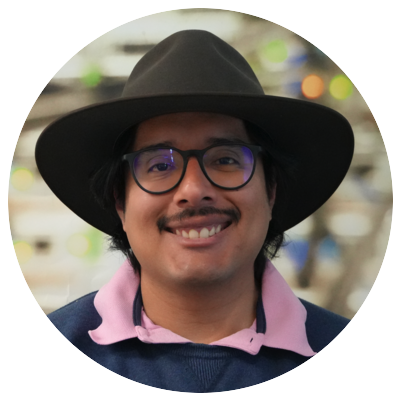
\includegraphics[width=2.8cm]{assets/jorge_c.png}\\[.5em]
  {\small\textbf{Jorge Luis Gálvez Vallejo}}\\{\footnotesize NCI \textperiodcentered\ ANU}
  \vfill
  {\large\color{cookieAccent}\textbf{¿Preguntas?}}\par
  \vspace{.3em}
  {\footnotesize jorge.galvezvallejo@anu.edu.au}
\end{frame}

\end{document}
